\documentclass[utf8,largesmallcaps,intlimits,widermath,sharecounter,backref,nobreak,definition=marks,numbers,noparts]{rtthesis}

\usepackage{mythesis}
\usepackage{tikz}
\usetikzlibrary{calc,angles,quotes,shadings}
\usetikzlibrary{calc,angles,quotes}
\usepackage{footmisc}

\usepackage{hyperref}

\begin{document}
\selectlanguage{english}

\frontmatter
\maketitle

\begin{abstract}[english]
  This thesis presents a comparison between different algorithms for optimal scanline voxelization of 3D models.
As the optimal scanline relies on line voxelization, three such algorithms were evaluated.
These were \textit{Real Line Voxelization} (RLV), \textit{Integer Line Voxelization} (ILV) and a 3D Bresenham line drawing algorithm.
RLV and ILV were both based on voxel traversal by \citeauthor{voxeltraversal}.
The algorithms were evaluated based on runtime and the approximation error of the integer versions, ILV and Bresenham.
The result was that RLV performed better in every case, with ILV being 20-250\% slower and Bresenham being 20-500\% slower.
% The timings were from different models and voxel resolutions.
The error metric used was the Jaccard distance and generally started at 20\% and grew up towards 25\% for higher voxel resolutions.
This was true for both ILV and Bresenham.
The conclusion was that there is no reason to use any of the integer versions over RLV.
As they both performed and approximated the original 3D model worse.

\end{abstract}

\begin{acknowledgments}
  I would like to thank my supervisors at Mindroad, Åsa Detterfelt and Jens Ogniewski, for guiding me through this thesis. I would also like to thank my colleagues at Mindroad for the great company during our breaks. A thanks also goes out to my examiner Ingemar Ragnemalm, both for the help provided during the thesis, but also for the great courses he provided during my studies. A special thanks goes out to my family for all their love and support during my education.

  \addvspace{1em}
  \begin{flushright}
    \textit{%
      Linköping, June 2020\\
      Tim Håkansson%
    }
  \end{flushright}
\end{acknowledgments}


\tableofcontents
% \begin{notation}
%   \centering

%   \begin{notationtabular}{Några mängder}{Notation}{Betydelse}
%     $\naturals$ & Mängden av naturliga tal \\
%     $\reals$ & Mängden av reella tal \\
%     $\complexes$ & Mängden av komplexa tal \\
%   \end{notationtabular}

%   \begin{notationtabular}{Förkortningar}{Förkortning}{Betydelse}
%     \abbrARMA\index{ARMA@\abbrARMA!abbreviation} & Auto-regressive moving average \\
%     \abbrPID\index{PID@\abbrPID!abbreviation} & Proportional, integral, differential (regulator) \\
%   \end{notationtabular}
% \end{notation}


\mainmatter

\chapter{Introduction}\label{cha:intro}
This chapter gives the reader an introduction to voxels, its uses and ways to create voxels from a model.
It also serves the purpose of motivating the thesis, as well as describing the problem it is out to solve.
Finally, it defines the delimitations of the thesis and presents the company, at which this thesis was conducted at.

\section{Background}
In computer graphics, a 3D model is built up of triangles which describes the surface of the model.
This means it does not store any information to represent the inside of the model.
In order to represent the inside, a volumetric data structure is needed.
Usually, this is done by storing \textit{voxels} in a uniform 3D grid.
A voxel can be described as data at a position in a grid.
This can be any form of data, such as occupancy, color, material or density.

% \textit{Voxel} is a word that has a lot of meaning in computer graphics.
% The simplest form of a voxel is a cube in a 3D-environment, but other representations of voxel data also exist.
% One such representation is marching cubes~\cite{marching-cubes}, where voxels are defined as density functions to a surface.
% This can create smooth surfaces from volume data, which has its uses in medical imaging~\cite{marching-cubes} and 3D-terrain~\cite{marching-cubes-terrain}.

As voxels are just a way to represent volumetric data, they have been used in a wide range of applications, such as global illumination~\cite{crassin-VCT}, medical imaging~\cite{marching-cubes,voxel-medicin} and collision culling~\cite{voxel-collision}.
These applications either store a voxel representation of models (especially true for medical imaging) or need to convert models into voxels.
This process is called \textit{voxelization} and has been widely studied in the past.
Some methods for voxelizations include triangle-box intersection~\cite{SAT-voxelization}, rasterization~\cite{octree-voxelization} and depth buffer~\cite{depth-buffer}.

Recently, a study was published by \call{scanline-voxelization} proposing a new method to voxelize a model.
The basics of the method is to voxelize the model by performing line voxelization at different stages.
This method is the basis of this thesis and will further be called the \textit{optimal scanline}. 
% The authors used both real and integer line voxelization based on~\call{voxeltraversal}.
% These two will further be called \textit{Real Line Voxelization} (RLV) and \textit{Integer Line Voxelization} (ILV).
% They mentioned ILV was slightly more efficient ($\sim$3\%), but the actual data was not published.

\newpage

\section{Aim}
This thesis aims to do an investigation of how the line voxelization algorithm affects the performance of the optimal scanline.
This includes both floating-point and integer line voxelizations.

The thesis also investigates the approximation error caused by using the integer versions of the algorithm.
This was done in \cite{scanline-voxelization}, but the authors only compared the voxel count.
Which means if a voxel is moved somewhere else, it would not produce any error.
As such, this thesis aims to measure this error in another metric, which can describe those errors.

\section{Research Questions}
With the aim of the thesis defined, two research questions are formed as a baseline of the thesis.
These are presented below:
\begin{enumerate}
  \item \label{que:linealg} Which line voxelization algorithm performs best for the optimal scanline?
  \item \label{que:erroraprox} How great is the approximation error of the integer versions of the optimal scanline?
  % \item \label{que:combine} Can the different line voxelization be combined to improve performance and accuracy?
\end{enumerate}
A better performance in this case is defined as how fast the execution of the voxelization is.
It is not a metric of the error or the memory usage of the algorithms.

\section{Delimitations}
The implementation of the thesis ran on \textit{Amazon Web Services} (AWS), on a computer running Ubuntu 18.04 with an NVIDIA Tesla T4 graphics card with driver version 440.59.

The rendering of the voxelization was done using OpenGL.
As the focus was not on supporting older devices, the OpenGL version 4.6 was used.

The computing language of choice was CUDA, as such, other languages were not considered for the implementation.
Again, as there is no need to support older devices, CUDA 10.2 was used.

The line algorithms that were evaluated were limited to a voxel traversal algorithm by \call{voxeltraversal}, its integer version and Bresenham.
As Bresenham is predominantly a 2D line drawing algorithm, it was extended to 3D using a method proposed by \call{3d-bresenham}.

The evaluations were also limited to three different models and voxel grid resolutions between 128-2048.

\newpage

\section{Mindroad}
This master thesis was conducted on behalf of MindRoad. 
MindRoad is a software company which specializes in embedded systems, web development and mobile applications. 
They also provide courses in software development, such as C++, Python, GPU-programming, Linux and driver development. 

\chapter{Background}\label{cha:theory}
This chapter serves the purpose of giving the reader a better understanding of central concepts throughout the thesis.
It will give an introduction to GPU-programming, AWS, voxelization and raycasting.

\section{GPU-Programming}
In GPU-programming, there are two different subjects to discuss, rendering and computing.
Rendering is where the GPU performs calculations, which results in some visual output.
This most often means taking triangles, performing different transformations on them and then drawing them to a screen.
Computing is similar, but instead of resulting in graphics on a screen, the results are stored in video memory as data.
This is useful when algorithms can make use of the GPU's parallelization.

In order for the GPU to do any form of calculations, an API is needed to interact with it.
For rendering, there are API:s such as OpenGL, DirectX and Vulkan.
API:s used for computing include CUDA and OpenCL.
All the rendering API:s above also support computing, but it is not what their general use is.

The chosen API:s for this thesis were OpenGL and CUDA, and are presented in the next sections.

\newpage

\subsection{OpenGL}
\textit{OpenGL}~\cite{opengl-about}, short for Open Graphics Library, is technically not an API but an open specification which defines functions used for 2D and 3D graphics.
As it is a specification, there are implementations for most platforms, including Windows, Linux, MacOS\footnote{OpenGL is currently deprecated (but still works) on Apple devices in favor of Metal~\cite{macos-opengl,ios-opengl}\label{fn:apple-depricated}}, Android and iOS\footref{fn:apple-depricated}.

To render with OpenGL, shaders are used to transform and color primitives, such as triangles.
The shaders are, in a sense, programs which are executed on the GPU.
When rendering a model, the GPU can run these shaders in parallel either per vertex, triangle or pixel, depending on the shader.
These are coded in GLSL, which supplies the developer with a wide range of vector math functions. 

OpenGL requires two shader programs in order to operate, the vertex and fragment shader.
The input to the vertex shader is, of course, vertices.
Often these vertices contain a position, normal and texture coordinate, and define a corner of a triangle.
The vertex shader then performs transformations on the vertices in order to move or in any way alter the triangles.
The result is then sent to a rasterizer, which turns these triangles into fragments.
These fragments are then the input of the fragment shader.
In simplest terms, fragments are pixels on the screen before they have been processed by the fragment shader.
The fragment shader is then able to perform calculations which changes the color of the fragment.
This can be based on normals, light positions, distance to the camera, etc.
The resulting color is then the color of the pixel on the screen.

There are two more programmable shaders in OpenGL, tessellation and geometry.
These are not required to render to the screen and will therefore not be discussed further in this thesis.

\subsection{CUDA}
\textit{CUDA} is an API for performing general computing on a GPU.
This API is being developed by NVIDIA and is only available on NVIDIA GPU:s.
However, it is cross-platform in terms of operating systems, as it is supported on Windows, Linux and MacOS.

CUDA is designed as a C/C++ extension and compiles using \textit{NVIDIA CUDA Compiler} (NVCC).
This compiler in turn makes use of a host compiler (such as g++) in order to compile the C/C++ code~\cite{nvcc}.
As such, there should not be any performance difference in the CPU code by using NVCC.

CUDA also has two different API:s which the developer can interact with, the driver and the runtime API.
The difference between them is minor, runtime CUDA is higher-level and is able to link the CUDA kernels into the compiled executable.
Kernels are basically CUDA programs, much like shaders are OpenGL programs.
The driver API on the other hand is lower-level and requires the program to read the CUDA kernels from an externally compiled cuda binary.

\newpage

\section{Amazon Web Service}\label{s:aws}
AWS~\cite{aws} is a set of cloud computing services provided by Amazon.
These services can provide the user with GPU computing, database management, cloud storage and many more services.

To interact with these services the protocol SSh is used.
This provides a way of connecting to a server with a terminal interface.
A problem with this, for the thesis, is that rendering is required to test the voxelization results.
In order to get a graphical interface on an AWS, Thinlinc~\cite{thinlinc} was used.
ThinLinc is a software which runs a desktop environment on a server and transfers the display over a network.
However, ThinLinc in itself does not support 3D hardware acceleration, which is needed by OpenGL.
As such, VirtualGL~\cite{virtualgl} was used when running the voxelization over ThinLinc.
This enables ThinLinc to run OpenGL with 3D hardware acceleration.
To run a program with VirtualGL simply prepend the program with \texttt{vglrun}.
For example, run \texttt{vglrun glxgears} to run the Linux GLX demo in ThinLinc.

\section{Voxelization}
In 2D, the process of turning triangles and other geometrical shapes into pixels is called \textit{rasterization}. 
Rasterization is required to render shapes onto a screen, as monitors cannot handle continuous shapes and have to discretize them into pixels.
An example of rasterization can be seen in \figref{fig:rasterization}.
Voxelization is the 3D version of rasterization, where instead of marking pixels in a 2D plane, it marks voxels in a 3D space.
Recall that a voxel can store any form of data, be it color, material or density.
What is stored is dependent on the use case of the voxels. 
In this thesis, only occupancy is stored, that is if the voxel exists or not.

\input{fig/rasterization.fig}

With voxelization defined there are two other topics that need discussing.
The first of which is if the algorithm supports surface or solid voxelization.
\textit{Surface voxelization} means the algorithm only voxelizes the outer surface of the model, and therefore leaves the voxelization with an empty interior.
\textit{Solid voxelization} is the opposite of that, filling the interior with voxels.
In this thesis, only surface voxelization will be considered, due to the optimal scanline only supporting it.

The other topic is the \textit{connectivity} of the voxelization.
There are three types of connectivity in a 3D voxelization, 6-, 18- and 26-connected.
The number signifies how many possibilities there are for two voxels to be considered connected.
A 2D example is seen in \figref{fig:connectivity}, where it is either 4- or 8-connected.
Similarly in 3D, two voxels are 26-connected if they share either a face, an edge or a corner between them.
Two voxels are 18-connected if they share a face or an edge between them.
Finally, two voxels are 6-connected if they share a face between them.
The authors of the optimal scanline claim the method can produce any voxelization connectivity, but mainly focuses on 6-connected. However, for the scanlines to work, 6-connected line voxelization is required.

\input{fig/connectivity.fig}

\section{Raycasting}
\textit{Raycasting} is a rendering technique where lines, often called rays, are being sent out from the camera.
If these rays intersect with an object in the world, that part of the object should be visible on the screen.
Information such as color, depth and material of the object can be retrieved by looking at where the ray intersected.

An early example of raycasting is its use in Wolfenstein 3D~\cite{wolf3d}.
In this game, a ray is being sent out for each column of the screen.
If a ray hits a wall, the game renders a vertical line with the height depending on the distance to the wall.
The color of the pixels in the line is then dependent on the texture of the wall.

Nowadays, raycasting can be performed for each pixel on the screen.
That is, for each pixel, send out a ray from the camera and color the pixel depending on what its ray intersects with.
As such, there is no need to perform any mesh rendering and only objects that are visible are being rendered.
For some use cases, this might be an optimal solution.
It is however an expensive operation if the use case is to render highly detailed triangle meshes, since it is difficult to find which triangle the ray intersects with.
This is because there are potentially thousands of triangles per model and millions of rays to test. 
Cases where raycasting is better to use are voxel grids, as there are algorithms to traverse it without evaluating every voxel.
One such technique is called \textit{raymarching} which marches through all voxels the ray goes through.
This is then terminated when a voxel is found or when the ray exits the scene.

\chapter{Theory}\label{cha:theory}
This chapter presents the literature used in order to answer the research questions.
It starts off with defining line voxelization and the three algorithms used.
Then the optimal scanline is presented together with other voxelization techniques.
Finally, some error metrics are presented, one of which is used as part of the final results.

\section{Line Voxelization}
\textit{Line voxelization} is a way of generating voxels based on a 3D line.
This is needed for the optimal scanline method to work, as this is how the scanlines are generated. 
In this thesis, line voxelization defines all voxels in a grid being touched by a line. 
This is similar to how lines are drawn to a screen in 2D.
An example of line voxelization can be seen in \figref{fig:line-voxelization}.
To determine which voxels are touching the line, three algorithms are introduced in the upcoming sections. 

\input{fig/line-voxelization.fig}

\newpage

\subsection{Real Line Voxelization}
\call{voxeltraversal} proposed a method of ray marching voxels in a uniform grid. 
This can also be used to voxelize lines and will further be called \textit{Real Line Voxelization} (RLV).
The basis of the algorithm is the line equation
$$p = p_0 + vt,$$
where $p$ is a position on the line, $p_0$ is the start position of the line, $v$ is the direction of the line (normalized) and $t$ is how much the direction is scaled.

When the algorithm starts, it initializes $t$ as
$$t_x = \frac{p_{1,x} - p_{0,x}}{v_x},$$
where $p_{1,x}$ is the x-position of the next voxel in the x-axis, as seen in \figref{fig:next-voxel}.
This is calculated similarly for each component of $t$.
Each iteration of the algorithm evaluates $t_{min}$ as $min(t_x,t_y,t_z)$.
Let's assume $t_{min} = t_x$.
This means the next voxel is in the x-direction.
Again, from \figref{fig:next-voxel}, $p_{1,x}$ is closer to $p_0$ compared to $p_{1,y}$ and therefore has a smaller $t$ value.
This means the next voxel would be placed to the right of $p_0$.
The $t$ for the next iteration is calculated by subtracting all of its components by $t_{min}$.

Finally assign 
$$t_x = \frac{|p_{i,x} - p_{i-1,x}|}{v_x} = \frac{1}{v_x},$$
where $p_{i,x}$ is the x-position of the $i$'th voxel in the x-direction.
Here the grid is assumed to have a voxel size of 1, meaning $|p_{i,x} - p_{i-1,x}| = 1$.
After this the iteration is restarted.
The iteration is then terminated when the sum of all $t_{min}$ exceeds the length of the line.

\input{fig/next-voxel.fig}

\newpage

\subsection{Integer Line Voxelization}
\textit{Integer Line Voxelization} (ILV) follows the same structure as RLV except it avoids the floating-point arithmetics and divisions.
The changes needed to avoid floating-points are adapted from \call{scanline-voxelization}.

Having RLV as a basis, ILV requires three changes.
Firstly, the initial $t$ is calculated from the center of the start voxel, which means 
$$p_{1,x} - p_{0,x} = \frac{1}{2},$$
and therefore
\begin{equation*}
\left\{
\begin{aligned}
    t_x &= \frac{1}{2 \Delta X} \\
    t_y &= \frac{1}{2 \Delta Y} \\
    t_z &= \frac{1}{2 \Delta Z}
\end{aligned}
\right.
,
\end{equation*}
where $\Delta X$ denotes the length of the line in the x-axis.
$\Delta Y$ and $\Delta Z$ are defined similarly.

Secondly, since only the relative sizes of $t$'s components are needed, the equation can therefore be multiplied with 
$$2 \Delta X\Delta Y\Delta Z,$$
to avoid fractions.
As such, the integer version of $t_x$ is denoted $T_x$ and can be described as
\begin{equation}\label{eq:Tx}
  T_x = \Delta Y\Delta Z.
\end{equation}
$T_y$ and $T_z$ are described similarly.

Lastly, the iteration of the algorithm follows RLV, replacing $t$ with $T$, but the assignment to $t_x$ in the end is instead 
$$T_x = 2 \Delta Y\Delta Z,$$
if $T_{min} = T_x$.
This follows \equref{eq:Tx}, but multiplied with 2.
The reason is that before $T$ was calculated to traverse half a voxel, multiplying it by 2 then traverses a whole voxel.

\subsection{3D Bresenham Algorithm}
The 3D version of the \textit{Bresenham} algorithm presented by \call{3d-bresenham} follows the original by \call{bresenham} rather nicely.
The 3D algorithm starts off with a few assumptions about the line,
$\Delta X \ge \Delta Y \ge 0$ and $\Delta X \ge \Delta Z \ge 0$, these are defined the same as in the previous section.

In the original Bresenham an error in the y-axis is initialized to
$$e_y = 2 \Delta Y - \Delta X.$$
Then for each iteration, if the current $x$ is greater than $X_1$, terminate the iteration.
Otherwise set the current voxel and increment $x$ by one.
Following that, check if the error of the line is greater than 0.
If it is, increase $y$ by one and decrease the error, otherwise increase the error.
Then restart the loop.
The change in the error is defined as

\begin{equation*}
\left\{
\begin{aligned}
  e'_y &= e_y + 2 (\Delta Y - \Delta X) &, e_y \ge 0\\
  e'_y &= e_y + 2 \Delta Y &, e_y < 0 \\
\end{aligned}
\right.
.
\end{equation*}

To extend the algorithm to 3D, \citeauthor{3d-bresenham} added another error, $e_z$, which kept track of when $z$ should increase.
This works the same way as $e_y$ and is evaluated after $e_y$.
A pseudo code of the algorithm can be found in \appref{app:3dbresen}.

\section{Model Voxelization}
As mentioned in the introduction, voxelization is a way of turning a 3D model or scene into voxel data.
This can be done in a wide range of ways and is still being researched today.
Four such techniques, two of which are based on the optimal scanline, are presented in the following sections.

\subsection{Floating-Point Optimal Scanline}\label{sss:vox_optscan}
One of the more recent works in voxelization include work done by \call{scanline-voxelization}.
This algorithm, called optimal scanline, uses line voxelization as its core concept.
All its calculations are done for each triangle of the model.
The algorithm first sorts the vertices of a triangle based on its most dominant axis.
This axis is defined as the x-, y- or z-axis which most aligns with the triangle's normal.
It can be determined by choosing the axis with the greatest absolute value of the normal's components.
That is, choose the axis which matches $max(|n_x|, |n_y|, |n_z|)$, where $n$ is the normal of the triangle.
The dominant axis will further be assumed to be the z-axis.

With the vertices of the triangle sorted, it performs line voxelizations between each of the vertices using RLV.
This results in all the edges of the triangle being voxelized.

In order to fill the interior of the triangle, it splits the edges into slices in the z-axis.
Where each edge has the same integer z-value.
Then, for each slice, perform 2D line voxelization between the edges of the triangle.
This is shown in \figref{fig:real-optimal-scanline}.
The figure also shows that not every edge voxel needs to contain a scanline endpoint.
That is where the optimal keyword of the algorithm comes in.
The authors propose a theorem stating that, there exists a distance, $l$, where there cannot exist a voxel between two parallel lines.
This distance can be seen in \figref{fig:scanline-distance}.
Intuitively, the distance can be seen to be the length of the voxel's diagonal projected onto the scanline direction, $d_{sl}$.
Furthermore, the length, $l$, can be calculated as $|d_{sl,x}| + |d_{sl,y}|$.
To prove this the scanline can be classified into four cases, all the combination of the signs of $d_{sl}$. The result is the four following equations:
\begin{equation*}
\left\{
\begin{aligned}
  l &= ((0,1) - (1,0)) \cdot d_{sl}\hspace{1cm},d_{sl,x} < 0 < d_{sl,y}\\
  l &= ((1,0) - (0,1)) \cdot d_{sl}\hspace{1cm},d_{sl,y} < 0 < d_{sl,x}\\
  l &= ((0,0) - (1,1)) \cdot d_{sl}\hspace{1cm},d_{sl,x}, d_{sl,y} < 0\\
  l &= ((1,1) - (0,0)) \cdot d_{sl}\hspace{1cm},0 < d_{sl,x}, d_{sl,y}\\
\end{aligned}
\right.
\end{equation*}
The values $(0,0)$, $(1,1)$, $(1,0)$ and $(0,1)$ are the corners of the voxel.
They are used to calculate the diagonal that aligns with $d_{sl}$.
Calculating the dot product of each of the equations results in $l = |d_{sl,x}| + |d_{sl,y}|$.

\input{fig/real-optimal-scanline.fig}
\input{fig/scanline-distance.fig}

\newpage

\subsection{Integer Optimal Scanline}\label{ss:integer-optimal-scanline}
The way integer voxelization of the optimal scanline is handled is a bit different from the floating-point one. 
Since the scanline direction and the scanline length are both floating-points, these cannot be used.
Instead, it makes use of an iterative approach, where it steps through the edge voxels of the triangle until the voxel is too far away from the previous scanline. 
How exactly it was derived can be found in~\cite{scanline-voxelization}, but the final theory is presented below (assuming z is the most dominant axis).

To start off, two boundary variables are defined, called $C_{lower}$ and $C_{upper}$.
These are defined as
\begin{equation*}
  \left\{
    \begin{aligned}
      C_{lower} &= \Delta Y X^a - \Delta X Y^a - |\Delta X| - |\Delta Y|\\
      C_{upper} &= \Delta Y X^a - \Delta X Y^a + |\Delta X| + |\Delta Y|
    \end{aligned}
  \right.,
\end{equation*}
where ($X^a$, $Y^a$) and ($X^b$, $Y^b$) are the endpoints of the previous scanline and $\Delta X = X^b - X^a$, $\Delta Y = Y^b - Y^a$.
Each iteration, the algorithm steps the edge voxelization by one voxel and calculate a variable called $C_k$ to be
$$ C_k = \Delta Y X_k - \Delta X Y_k, $$
where ($X_k$, $Y_k$) is the k'th voxel on the edge, with k=0 being the previous scanline endpoint.
If this variable is outside the boundaries, $C_{lower}$ and $C_{upper}$, the voxel is too far away from the previous scanline and $(X_{k-1},Y_{k-1})$ is chosen as the next scanline endpoint. 
This iteration is performed separately for both the edges.
As a triangle has three edges and not two, the voxels on the edge from $v_1$ to $v_2$ are merged with the voxels on the edge from $v_2$ to $v_3$.
Those two edges are therefore counted as a single edge.

\subsection{Rasterization}
Another technique used for surface voxelization utilizes the GPU rasterizer in order to optimize the voxel generation.
One such technique was presented by \call{octree-voxelization}.
The basic idea is that, for every triangle in the model, find the triangle's most dominant axis and render it from that direction. 
In practice, this means swapping the dominant axis with the z-axis in a vertex shader.
The triangle is then sent to the rasterizer which outputs fragments of the triangle.
The voxel coordinate is then simply the position of the fragment and its depth value.
Then the axes are swapped back from before in order to place it correctly in the scene.
Finally it writes the coordinate to a 3D texture which stores the voxel data.
Note that all rasterization is done in a framebuffer with the same width and height as the voxel grid resolution.
There are however problems with the algorithm creating holes in the voxelization in some instances.
It can be resolved by using a technique called conservative rasterization.
This involves marking all fragments which are touched by the triangle. 


% \subsection{Triangle-Box Intersection}
% Triangle-box intersection is another method of voxelization that was proposed by \call{SAT-voxelization}.
% The main idea of the method is, as its name implies, performing intersection tests between the voxels and the triangles.
% In order to minimize the amount of tests, a few optimizations are done.
% The first of which is classifying the type of triangle it is, be it a 1D line, a 2D triangle or a 3D triangle.
% These are further classified to their respective dominant axis.
% All the triangles of the model are then sorted so that they are grouped in their classes. 
% This makes it so that most of the GPU threads are performing the same tasks without branch divergence.
% Another optimization is that a triangle has at most three voxel thickness in the most dominant axis.
% This could reduce the amount of tests needed significantly.

\newpage

\subsection{Depth Buffer}
One way of performing solid voxelization is to make use of the depth buffer \cite{depth-buffer}.
This is done by rendering the entire model from six different directions, positive x, y and z, and negative x, y and z.
In these rendering steps, only the depth buffer is needed.
Then the voxelization is defined as all voxels which are within all the depth buffers. 

One way to do this, is to iterate through the entire grid and marking all voxels which are within the buffers as occupied.
This is however rather slow for higher resolutions, as the complexity grows cubically.
Another way would be to choose one axis, let's say the z-axis, and iterate through its buffer x- and y-coordinates.
Then for each coordinate, there is a minimum and maximum z-position which is determined by the two depth buffers in the z-axis.
This means the algorithm only needs to iterate through these two values instead of all the z-values.
As most models do not fill the entire voxel grid, this reduces the runtime of the algorithm in the average case.

One obvious problem of the algorithm is that it needs to render the object six times to voxelize it.
For convex shapes, this can be reduced to two, as the shape can be fully described by rendering it from the front and back. 

\section{Error Analysis}\label{s:error}
Calculating the approximation errors can be done using several methods.
The choice of method depends on the use case.
This thesis presents two different methods to analyze the error.
These are relative error, the one used in~\cite{scanline-voxelization}, and the Jaccard distance.

\subsection{Relative Error}
The \textit{relative error} can be described as
\begin{equation*}
  e_{re} = \frac{|x - y|}{|x|} = \Big|\frac{x - y}{x}\Big|,
\end{equation*}
where $x$ is the actual value and $y$ is the approximation.
This was the method used by \call{scanline-voxelization}, where they set $x$ to the total voxel count of the floating-point version and $y$ to the total voxel count of the integer version.
A problem with this is that if a voxel is moved to another location, the error would be considered 0.
This can be seen in \figref{fig:relative-error}, where the relative error of the voxel count is 0.
Therefore, a different error metric is required in order to describe this error.

\input{fig/relative-error.fig}

\newpage

\subsection{Jaccard Distance}\label{ss:mae}
The \textit{Jaccard distance} is an error metric which aims to measure differences in sets.
It is derived from  the Jaccard similarity presented in \cite{jaccard}, where it instead measures how similar two sets are.
The Jaccard similarity is defined as the size of the intersection divided by the size of the union of the two sets.
This results in a value between zero and one, which can be interpreted as a percentage of how similar two sets are.
The Jaccard distance is defined as one subtracted by the Jaccard similarity.
It can also be defined as the symmetric difference divided by the union of the two sets.
Both of which are equivalent.

\chapter{Method}\label{cha:method}
This chapter describes the implementation and application of the theory in more detail.
As such, it will build upon the literature in order to more precisely describe how the project was implemented.
The chapter will also give a description of how the evaluation of the different algorithms was performed.

\section{Implementation}
The full source code of the project can be found at \cite{source-code}.
The implementation was done in C++ with OpenGL and CUDA.
CUDA handled the voxelization and OpenGL was used to render the results of it.
The project was implemented in Linux, but can of course be ported to other platforms.
The implementation details which were not covered in the literature will be explained in the following sections.

\subsection{CUDA-OpenGL Interoperability}
During development, some form of visual feedback was required in order to verify and debug the results of the voxelization.
As such, a CUDA-OpenGL interoperation had to be implemented.
This meant creating a 3D texture in OpenGL and binding it to CUDA in order to write to it.
A simplified source code of this can be seen in \appref{app:cuda-opengl-inter}, which is adapted from~\cite{cuda-opengl-Interoperability}.
This method links the memory of the 3D texture to a CUDA array, meaning no data is duplicated.
This is required, as texture sizes of up to 8 GB were used.

\vfill

\subsection{Floating-Point Voxelization}
The first implementation detail that needs to be explained is how the scanline direction, $d_{sl}$, as shown in \figref{fig:scanline-distance}, was calculated.
Let's call the three vertices of a triangle $v_1$, $v_2$ and $v_3$, which are sorted in the most dominant axis (assumed to be the z-axis).
The scanline direction was calculated in two different ways, depending on how the vertices were positioned.
First, if all vertices were in the same z-slice, any direction would sufficed.
In the implementation, the edge between $v_1$ and $v_3$ was chosen.
If the vertices were not in the same z-slice, the gradient of the triangle with respect to $z$ was used.
This was calculated by first solving the plane equation for $z$:
$$ D = n_x x + n_y y + n_z z \rightarrow z = \frac{D - n_x x - n_y y}{n_z},$$
where $n$ is the normal of the triangle and $D$ describes the position of the plane.
The gradient was then the partial derivatives of the equation with respect to $x$ and $y$:
$$d = (\frac{-n_x}{n_z}, \frac{-n_y}{n_z})$$
Which was the resulting scanline direction.

In both cases, the direction also needed to be normalized, meaning the final direction was
$$d_{sl} = \frac{d}{|d|}.$$

Each iteration of the algorithm, two scanline endpoints were calculated by reverse projecting the scanline direction onto the triangle's edges. 
The scanline direction was scaled by $l_i$, which was increased by $l$ each iteration.
Recall from the theory that $l = |d_{sl,x}| + |d_{sl,y}|$.
Using the reverse projection, the endpoints were calculated as
\begin{equation}
v_p = v_1 + d_e\frac{l_i}{d_e \cdot d_{sl}},
\label{eq:inverse-projection}
\end{equation}
where $d_e$ is the normalized direction of the edge it projects to.
Note that this only works with the edges from $v_1$ to $v_2$ and $v_1$ to $v_3$.
So a special case was needed for the edge from $v_2$ to $v_3$.
This was solved by recalculating $v_2$ such that 
\begin{equation*}
  \left\{
    \begin{aligned}
      0 &= (v^\prime_2 - v_1) \cdot d_{sl} \\
      v^\prime_2 - v_2 &= (v_3 - v_2)t 
    \end{aligned}
  \right.
  .
\end{equation*}
That is, $v^\prime_2 - v_1$ is perpendicular to $d_{sl}$ and $v'_2 - v_2$ is parallel with $v_3 - v_2$.
An example of this can be seen in \figref{fig:triangle-v2}.
Solving the equation resulted in
$$
v^\prime_2 = v_2 + (v_3 - v_2)\frac{(v_1 - v_2) \cdot d_{sl}}{(v_3 - v_2) \cdot d_{sl}}.
$$
This was used instead of $v_1$ in \equref{eq:inverse-projection}, when projecting to the edge between $v_2$ and $v_3$.
\input{fig/triangle-v2.fig}

\subsection{Integer Voxelization}\label{ss:meth-integer-vox}
In the integer version there were two edge cases which created holes in the voxelization.
In order to solve these problems first recall the values $C_{lower}$, $C_{upper}$ and $C_k$ from the theory in \secref{ss:integer-optimal-scanline}.

The first problem occurred when a new slice was started and an example is shown to the left in \figref{fig:integer-miss}.
More specifically, it occurred when the next voxel was behind the current scanline, meaning it should have been included in it.
This was resolved by checking if the value of $C_1$ was on the other side of $C_0$ relative to $C_{end}$.
That is, if $C_0 < C_1 < C_{end}$ or $C_{end} < C_1 < C_0$.
Here $C_{end}$ is defined as the $C_k$ of the last voxel on the triangle's edge.
To test if the two values were on different sides, following equation was evaluated:
$$ (C_1 - C_0) * (C_{end} - C_0) \leq 0.
$$
If this condition was met, either $C_{upper}$ or $C_{lower}$ was set to $C_0$ depending on if $C_{end}$ was greater or less than $C_0$ respectively.
This was done in the same step as when the next endpoint for the scanline is calculated.

The other case where holes occurred was when $(X_1, Y_1)$ for both edges were on different sides of the scanline.
This sometimes happened for triangles which had a very acute angle at $v_1$.
An example of this can be seen to the right in \figref{fig:integer-miss}.
This problem was similarly detected as before by
$$ (C^a_1 - C_0) * (C^b_1 - C_0) \leq 0,$$
where $C^a_1$ and $C^b_1$ are $C_1$ for the two edges.
When this was the case, $\Delta X$ and $\Delta Y$ were set similarly to how the scanline direction was chosen for the floating-point version.
That is, the gradient of the triangle was calculated, but the division by $n_z$ was removed to avoid floating-point operations.
However, this resulted in a scanline direction and not a difference between scanline endpoints.
So it was also rotated by 90$\degree$, as the scanline should always be perpendicular to the scanline direction.
The result was $\Delta X = N_y$ and $\Delta Y = -N_x$, where $N$ is the unnormalized normal of the triangle.
These values were then used when determining the next scanline endpoints.

\input{fig/integer-voxel-miss.fig}

\subsection{Bresenham Algorithm}\label{ss:bresenham-problems}
Worth noting is that Bresenham only works when $\Delta X$ is positive and greater than $\Delta Y$ and $\Delta Z$.
To allow for negative directions, three changes were required.
First, whenever $x$, $y$ or $z$ increased by one, they were instead decreased by one if the difference was negative.
Another change was to set $\Delta X$, $\Delta Y$ and $\Delta Z$ to their absolute value.
Finally, the iteration was terminated when the x-position of the voxel equals $X_1$, where $X_1$ is the last x-position on the line.
This would however miss the last voxel on the line, which was resolved by setting the last voxel after the loop.

To solve the problem where $\Delta X$ has to be greater than the other differences, a variable which keeps track of this axis was introduced.
This variable will be called $A$ and was initialized to
\begin{equation*}
\left\{
\begin{aligned}
  A = 0 \hspace{1cm} &, max(\Delta X, \Delta Y, \Delta Z) = \Delta X \\
  A = 1 \hspace{1cm} &, max(\Delta X, \Delta Y, \Delta Z) = \Delta Y \\
  A = 2 \hspace{1cm} &, max(\Delta X, \Delta Y, \Delta Z) = \Delta Z \\
\end{aligned}
\right.
.
\end{equation*}
Then whenever the $\Delta X$ or $x$ was needed, instead the variable was indexed using $A$.
For example $\Delta [A]$, would give the greatest difference.
The indices of the other two axes was calculated by increasing $A$ by one and two respectively, and then taking the modulus 3 of them.

Another thing missing from the theory is that Bresenham is not 6-connected.
This can be seen in \figref{fig:bresenham-8}.
As the optimal scanline requires 6-connected lines in order to fill the interior, the Bresenham algorithm had to be modified to support this.
The first intuitive way to do this would be to add a voxel at $(x,y,z)$ whenever $y$ or $z$ increases in the algorithm.
This however, caused the voxelization to not follow the line correctly, as seen to the left in \figref{fig:bresenham-8}.
This was solved by checking if the error in $y$ was greater than $\Delta Y$, then instead of voxelizing the right voxel, voxelize the top voxel.
The result can be seen to the right in \figref{fig:bresenham-8}.
The same check was performed on the z-axis.
This modification of the algorithm in \appref{app:3dbresen} can be seen in \appref{app:3dbresen-4}.

The final problem with the Bresenham algorithm was that the integer version of the scanline algorithm required being able to get the next voxel in the line.
The problem was that the 6-connected Bresenham could generate up to three voxels each iteration.
One way to solve the problem would be to run one iteration of Bresenham and store all voxels generated in that iteration in a list.
Then the next time a new voxel is needed, return an unused voxel from the list.
The way it was solved for this thesis however, was to keep track of where the last voxel was returned in the iteration.
Then the next time a voxel was needed, the iteration resumed where it left off last.

\input{fig/bresenham-8.fig}

\input{fig/bresenham-4.fig}

\subsection{Voxel Rendering}\label{ss:voxel_rendering}
In order to test the results of the optimal scanline, some form of rendering was needed.
This thesis only considers rendering which results in cubes in a uniform grid.

One approach would be to iterate through the 3D texture on the CPU and render a cube for every existing voxel.
This would be bad for numerous reasons.
First off, the data created on the GPU would need to be copied over to the CPU, which creates significant overhead.
Especially since the data could get up towards 8 GB in size for the highest resolution.
Secondly, rendering all voxels (even occluded ones) would slow down the rendering significantly.

Another way would be to write each voxel coordinate to a list on the GPU when voxelizing the model.
The data could then be used in a geometry shader, where each coordinate is transformed into a cube.
This avoids the copying to the CPU and requires less data to store the voxelization, since only occupied voxels are stored.
It can, however, render the same voxel multiple times if the voxelization does not keep track of which voxels are already occupied.

Therefore, rendering the scene using raymarching was both deemed easier and a potentially faster method.
The data was not transferred between the CPU and GPU and only the visible voxels were rendered.

To perform the raymarching, it used the RLV algorithm to traverse the voxels.
In this case however, the line was not terminated when it reached the endpoint of the line segment, as it does not exist.
Instead it terminated when the line intersected with an existing voxel or when it had exited the voxel grid.

\section{Evaluation}
When performing the comparisons of the different line algorithms, several variable changes were considered in the experiments.

Firstly, multiple models were tested on, with ranging levels of detail.
The models that were used included the Blender monkey (also called Suzanne)~\cite{blender-monkey}, the Stanford bunny~\cite{stanford-rep} and the Stanford dragon~\cite{stanford-rep}.
These can be seen in \figref{fig:models}.
The triangle count of each model was 3936, 69451 and 871414 respectively.
Suzanne was also subdivided once in Blender~\cite{blender}, in order to increase the triangle count to 3936.

Secondly, the resolution of the voxel grid was varied for each model.
The resolution varied between 128-2048, incremented by powers of 2.
Due to GPU memory limits, resolutions greater than 2048 were not possible.

\input{fig/models.fig}

\subsection{Performance Analysis}
To profile the performance of the algorithms, CUDA events were used~\cite{cuda-profiling}.
To use the CUDA events, two timestamp events were created.
One of them was initialized before the kernel ran using the CUDA function \texttt{cuEventRecord}.
Then after the kernel ran, another event was initialized.
These timestamps were entirely handled by the GPU, meaning the CPU would not wait for the timestamps to be executed.
The function \texttt{cuEventSynchronize}, was used in order to wait for the events to be executed.
The time between two timestamps was then determined by the CUDA call \texttt{cuEventElapsedTime}.

\newpage

\subsection{Error Analysis}
The error was calculated for each of the resolutions, models and combinations of line voxelizations.
Meaning RLV was compared to both ILV and Bresenham, but ILV was also compared to Bresenham.

The comparison was done by first voxelizing using the first algorithm with the voxel value of 1.
Then the voxelization ran again with the other algorithm (with the same 3D texture). 
This time the voxel value was determined depending on the current voxel value in that position.
If the value at that position was 1 or 2, the value 2 was written, otherwise the value 3 was written.
The result was a voxelization where the intersection had value 2, the voxels only in the first algorithm had value 1 and the voxels only in the second had value 3.

To calculate the error, a simple CUDA kernel was created which iterated through the whole voxel space and summed up the amount of each of the values.
With these values the error could be calculated using the formulas in \secref{s:error}.

\chapter{Results}\label{cha:results}
Here the results of the thesis will be presented.
This includes figures of the voxelization, graphs of the performance and data of the error analysis.

\section{Voxelization}
The result of the floating-point voxelization can be seen in \figref{fig:voxelization}.
The same voxelization of the integer versions is shown in \figref{fig:voxelization-ilv} and \figref{fig:voxelization-bresenham}.
The figures show voxelizations between 16-512 resolution, but resolutions up to 2048 were possible.
However, due to the aliasing in the rendering, showing the result of such high resolution would be meaningless.

All the models in the voxelization were scaled to fit the voxel grid perfectly, without changing the aspect ratio of them.
More figures of the voxelizations can be found in \appref{app:voxelizations}.

\section{Performance Analysis}
The performance of each of the models can be seen in \figref{fig:performance-model}.
The same data is plotted for each of the algorithms in \figref{fig:performance-alg}.
Each data point is the average time to voxelize the models in a total of 100 iterations.
The raw performance data can be found in \appref{app:performance-data}.

One unsolved problem about the performance data is that the timings improved after iterating the voxelization multiple times.
As an example, \figref{fig:performance-runs} shows how the timings varied after a certain amount of iterations.
The time for a single voxelization decreased by around 50\%.
This will further be discussed in the next chapter.
Since the data seem to converge to a certain time, the average of the last 100 out of the 1000 iterations were used as the final measurement in the previously mentioned graphs.
% \begin{table}[ht]
%   \centering
% \begin{tabular}{l|l|lllll}
%   Model & Algorithm & 128 & 256 & 512 & 1024 & 2048 \\
%   \hline
% \multirow{2}{*}{Monkey} & ILV       & 20\% & 60\% & 56\% & 43\% & 32\% \\
%  & Bresenham & 40\% & 76\% & 59\% & 37\% & 20\% \\
% \hline
% \multirow{2}{*}{Bunny} & ILV       & 210\% & 231\% & 86\% & 35\% & 25\% \\
%  & Bresenham & 410\% & 420\% & 156\% & 69\% & 48\% \\
% \hline
% \multirow{2}{*}{Dragon} & ILV       & 215\% & 255\% & 250\% & 235\% & 133\% \\
%  & Bresenham & 448\% & 518\% & 495\% & 443\% & 234\% \\
% \end{tabular}
% \caption{Runtime increase for the integer versions relative to RLV. All values are rounded to the nearest whole number.}\label{tab:performance-data}
% \end{table}

% \FloatBarrier

\input{fig/voxelization.fig}

\voxelizationfig{bunny}{rlv}{Floating-point voxelization using RLV of the Stanford bunny at 16, 32, 64, 128, 256 and 512 resolution}{fig:voxelization}
\voxelizationfig{bunny}{ilv}{Integer voxelization using ILV of the Stanford bunny at 16, 32, 64, 128, 256 and 512 resolution}{fig:voxelization-ilv}
\voxelizationfig{bunny}{bre}{Integer voxelization using Bresenham of the Stanford bunny at 16, 32, 64, 128, 256 and 512 resolution}{fig:voxelization-bresenham}
\input{fig/performance-model.fig}
\input{fig/performance-alg.fig}

\input{fig/performance-runs.fig}

\FloatBarrier

\section{Error Analysis}
An example of the difference between RLV and ILV can be seen in \figref{fig:compare}. 
It shows a comparison where voxels are colored depending on if they exist in both voxelizations or only one of them.
More comparisons can be seen in \appref{app:compare-error}, where all models and resolutions between 16-512 are shown. 

The Jaccard distance between the different versions of the voxelizations can be seen in \tabref{tab:error-data}. 

\begin{figure}[h]
\centering
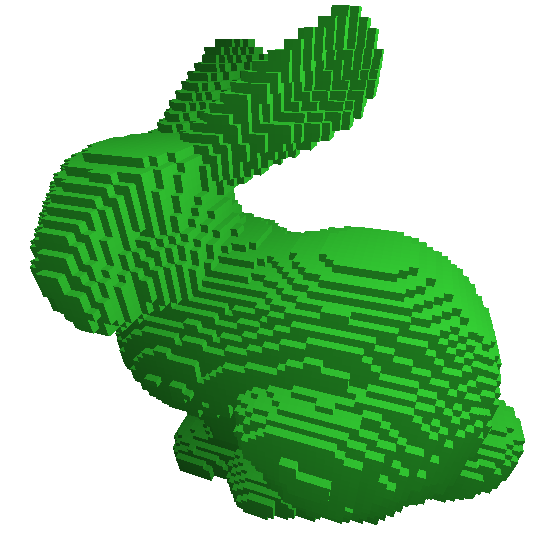
\includegraphics[width=0.3\textwidth]{fig/voxelization/bunny/bunny_rlv_64.png}
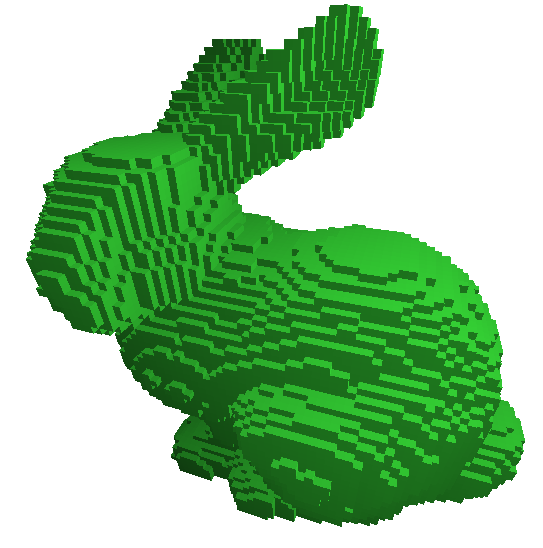
\includegraphics[width=0.3\textwidth]{fig/voxelization/bunny/bunny_ilv_64}
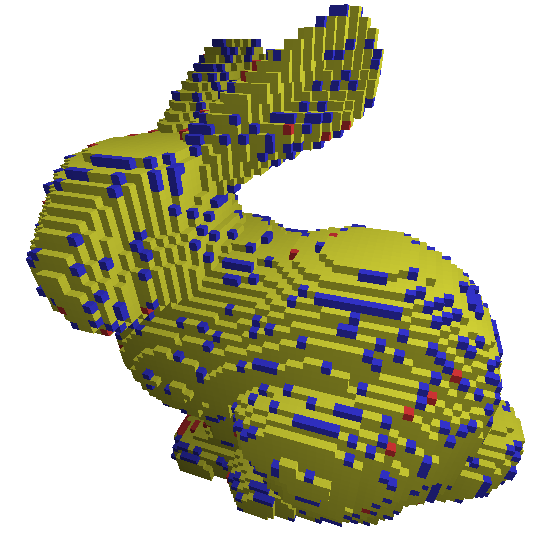
\includegraphics[width=0.3\textwidth]{fig/voxelization/bunny/bunny_rlv_ilv_64}
\caption{
  Difference between floating-point and integer voxelization.
  The left-most figure uses RLV, the middle uses ILV and the right-most is the union between them.
  The yellow voxels are in both versions.
  The red voxels are only in the RLV version.
  The blue voxels are only in the ILV version.
}\label{fig:compare}
\end{figure}

\begin{table}[h]
  \centering
\begin{tabular}{l|l|lllll}
  Model & Algorithm & 128 & 256 & 512 & 1024 & 2048 \\
  \hline
         & RLV/ILV & 21.63\% & 22.10\% & 22.51\% & 22.98\% & 23.53\% \\
  Monkey & RLV/Bre & 21.89\% & 22.30\% & 23.04\% & 23.67\% & 24.16\% \\
         & ILV/Bre & 4.72\% & 5.62\% & 5.58\% & 5.35\% & 5.21\% \\
  \hline
         & RLV/ILV & 19.65\% & 20.62\% & 22.12\% & 22.59\% & 22.8\% \\
  Bunny  & RLV/Bre & 19.66\% & 21.21\% & 22.30\% & 22.94\% & 23.21\% \\
         & ILV/Bre & 0.07\% & 4.57\% & 4.77\% & 5.59\% & 5.23\% \\
  \hline
         & RLV/ILV & 9.42\% & 15.65\% & 21.28\% & 21.87\% & 22.75\% \\
  Dragon & RLV/Bre & 9.42\% & 15.67\% & 21.40\% & 22.52\% & 23.29\% \\
         & ILV/Bre & 0.00\% & 0.05\% & 1.09\% & 3.84\% & 5.22\% \\
\end{tabular}
\caption{The Jaccard distance between the different algorithms, with varying models and resolution. Bre in the table is short for Bresenham. All errors are rounded to the nearest hundredth.}\label{tab:error-data}
\end{table}


\chapter{Discussion}\label{cha:discussion}
This chapter discusses the results from the method.
This includes explaining the given data and how the data changes depending on models and resolution.
It will also give a critical view of the method and explain why certain methods were used.
Finally, a discussion will be had about future improvements and research which can be done surrounding the thesis.

\section{Results}
This section discusses the results shown in the previous chapter.
It serves the purpose of explaining and evaluating the data gathered from the method.

\subsection{Performance of Models}
From \figref{fig:performance-alg} in the results, it can be seen that the voxelization generally takes longer with the increase in triangle count.
This makes sense, as having more triangles to process should increase the amount of time to voxelize. 
The timings of the models do however seem to converge towards the same value as the resolution increases.
This is likely due to the fact that even though there are less triangles in the monkey compared to the dragon, the monkey needs to generate more voxels per triangle.
Meaning the GPU cannot utilize its parallelism when less triangles are being voxelized.
This can be seen in \figref{fig:performance-alg} for RLV, where even though the dragon has ten times more triangles, it outperforms the bunny at higher resolutions.

\vfill

\subsection{Performance Between RLV and ILV}
Looking back at article of the optimal scanline~\cite{scanline-voxelization}, the authors claimed 
ILV was around 3\% faster than RLV. 
Again, the data was not published in the article.
This is however not consistent with the results of this thesis, where ILV was worse by between 20-250\%.
There could be several reasons for this.

First of, the article never states anything about the edge-cases in the integer version presented in \secref{ss:meth-integer-vox}.
Fixing these edge-cases caused some overhead, which they might not have had.

Secondly, much of the focus of the article was around the integer version and few details were explained about the floating-point version. 
This meant a lot of improvisation had to be done when implementing the floating-point version.
Therefore, it is possible it was implemented in a more efficient way.

Thirdly, there is of course a possibility that the authors skipped some optimization steps in the article.
This could be because they had a budget on the amount of pages they could write, or the full optimization steps were deemed too complicated for the article.

The results of my implementation are however reasonable considering the different complexities of finding the scanline endpoints.
In the floating-point version, all that had to be done is increasing the scanline length and calculating a reverse projection of the scanline direction.
The integer version required iterating through multiple voxels to find the endpoint. 
As such, it would make sense that the floating-point version required fewer calculations to find the endpoints.

\subsection{Performance Between ILV and Bresenham}
Since ILV and Bresenham use the same integer version, the performance difference is solely based on the line voxelization algorithm.
The original hypothesis was that Bresenham would improve performance, but looking at the data, this is not the case.

The big reason for this was the last problem described in \secref{ss:bresenham-problems}, that Bresenham could generate three voxels per iteration.
This meant that additional overhead was needed in order to get the next voxel in the Bresenham voxelization.
In ILV the same operations are performed no matter which direction the next voxel is in, but in Bresenham different calculations are done at different stages.
This resulted in Bresenham causing more branch divergence on the GPU, which caused a major slow down.

\subsection{Performance Data}
After analyzing the performance data, it was noted that the timings changed drastically when iterating the voxelization many times.
The reason for this is still unknown, but it is somehow caused by AWS.
This was discovered after testing the voxelization on normal desktop computers, which had none of these issues.
There are two hypotheses as to why this could happen.

One reason could be that the program ran over a network.
As described in \secref{s:aws}, to run the voxelization, ThinLinc together with VirtualGL was used.
This could potentially cause extra overhead which brings down the performance. 
It does however not explain why the CUDA performance is suffering from this, as VirtualGL only enables OpenGL 3D acceleration.
However as the implementation makes use of OpenGL textures, VirtualGL could still be the culprit.

The other hypothesis is that AWS allocates more resources as it is needed. 
Meaning the program does not run at full power until it has run for a certain amount of time.
This could explain the distinct performance boosts seen in \figref{fig:performance-runs} in the results.

Again, there is no conclusive answer as to why the performance increases, the reasons above are just speculations as to why. 

\subsection{Error Analysis}
\tabref{tab:error-data} in the results shows all the error data between the different voxelization algorithms.
The error between RLV and ILV grew as the resolution of the voxelization increased.
The same was true between RLV and Bresenham.
It seems like the error converges around 25\%, which is a considerable difference to the 2.5\% presented by \call{scanline-voxelization}.
Again, the error presented in the article is a relative error of the voxel count between the two voxelizations, which is different to the Jaccard distance.

An interesting data point is the error for the Stanford dragon.
In the lower resolutions the error was a lot less than the error for the other models.
This is likely due to the fact that the triangle count was much higher.
The result is that a lot of triangles were fully inside a voxel, meaning there could not be an error for those triangles.
For the triangles which were not fully inside a voxel, they generally spanned a total of 3-4 voxels and were therefore also prone to less error.
This is also consistent with the error increasing as the resolution increased.

Looking at \tabref{tab:error-data}, it can be seen that there was an error of up to 5\% between ILV and Bresenham.
As they both used the same underlying integer algorithm, it would seem odd that there was an error between them.
The error occured when the line touched more than two voxels.
That is, the line did not pass through the face of the voxels.
This is shown in \figref{fig:ilv-bresen-error}.
The ambiguity of which voxel should be chosen caused the two versions to generate slightly different voxelizations.
A potential fix for this would be to voxelize all the voxels touching the line, but this would most likely cause more edge-cases when finding the next scanline endpoint. 

\input{fig/ilv-bresen-error.fig}

\vfill

\section{Method}
This section serves the purpose of motivating and critically analysing the methods used in the thesis. 

% \subsection{CUDA Vector Math}
 
% Discuss that CUDA doesn't support vec2-4 by default.
% As such, this needed to be implemented manually.
% This might cause the performance to be less than optimal.

% \subsection{CUDA-OpenGL Interoperability}
% One thing of note with the CUDA-OpenGL interoperability is that it used OpenGL 3D textures when storing the voxelization in CUDA.
% As such, there is a possibility that the texture access might not be as fast as indexing a CUDA array.
% This would mean the performance might be impacted by using OpenGL.
% However, as this method was used for all performance tests, there should not be a problem with comparing the performance between algorithms.

\subsection{Performance Analysis}
To run the performance analysis, CUDA events were the choice for this thesis.
These events only measured the execution time of the kernel and did not include the time it took to launch it.
An alternative to this would be to use CPU timers.
This would give a more real depiction of how long the voxelization would take in a real environment, as it would include the launch time of the kernel.
However, this thesis is set out to measure the performance of the voxelization and including the launch time of the kernel was deemed unnecessary.

\subsection{Error Analysis}
There is also something to be said about how the error was measured.
As the Jaccard distance only calculates the amount of mismatched voxels, it is not a measurement of how well the general shape of the voxelizations matches.
As such, it should not be used for comparing dissimilarity of voxelizations between different models.
It is more of a metric to compare already similar data sets.
The results of using this method could therefore be misleading when saying the voxelization has an error of 20-25\%.
Such great error might leave the reader to believe the integer version is unrecognizable to the floating-point version.
This is however not the case as the general shape is preserved very well, and it is hard to visually see the error without a comparison figure. 

\section{Future Work}
As always with a project like this there is still room for improvements.
Some of those improvements are described in the following paragraphs.

Firstly, modify the Bresenham algorithm to perform better when retrieving the next voxel in the line.
The problem is that it performs different calculations depending on which axis it is currently evaluating.
One solution could be to add an additional error for the dominant axis.
This would then result in all axes performing the same calculations.
Then to get the next voxel iterate the different axes until a voxel is found.
To determine which axis to evaluate, a variable can be used to index the axes.

Secondly, analyze the error between the algorithms when performing a supercover line voxelization.
A supercover avoids the ambiguity of which voxel to voxelize when the line touches multiple voxels.
This is done by voxelizing all the voxels instead of choosing one of them.
Doing this could fix the problem with the integer versions generating different voxelizations due to the ambiguity.

% \begin{itemize}
%   \item Sort triangles based on their slope, in order to avoid branch divergence?
%   \item Investigate the performance improvements after running the voxelization a few times?
%   \item More models and details to better figure out what causes different levels of performance?
% \end{itemize}

\chapter{Conclusion}\label{cha:conclusion}
This chapter answers the research questions by summarizing the results and discussions.
It also gives a conclusive answer as to which algorithm one should use when implementing an optimal scanline algorithm.

\section{Research Questions}
The research questions presented in the introduction are reiterated and answered in the following paragraphs.

\begin{enumerate}
\item Which line voxelization algorithm performs best for the optimal scanline? 
\end{enumerate}
For all models and voxel grid resolution, the floating-point version, RLV, performed better.
ILV performed anywhere between 20-250\% worse compared to RLV.
Bresenham performed anywhere between 20-500\% worse compared to RLV.
Interestingly, ILV performed better than Bresenham in every case but two.
Although, the difference was not as dramatic as between RLV and ILV, except for a few outliers which performed way worse.

The reason for the big difference between the floating-point and integer versions was due to the complexity of finding the scanline endpoints.
For RLV, it was simply a case of increasing the length of the scanline direction and performing a reverse projection of the direction to the triangle's edges.
For ILV and Bresenham, finding the endpoints required iterating through the edge voxelizations and performing a boundary test based on the previous scanline and the current voxel.

The reason for ILV being faster than Bresenham had less to do with Bresenham being worse in general.
It had more to do with Bresenham not being able to step the line voxelization by one voxel each iteration.
This in turn required extra overhead to overcome.

\begin{enumerate}
\setcounter{enumi}{1}
\item How great is the approximation error of the integer versions of the optimal scanline?
\end{enumerate}
The error for the integer versions of the optimal scanline was determined to be around 20-25\%.
This was based on the Jaccard distance between RLV and ILV/Bresenham.
One outlier of the data was the dragon model, with 871414 triangles, where the error started at around 9\% for a voxel grid resolution of 128.
It however gradually grew as the resolution increased.
The reason was likely due to the triangles of the model being mostly within a single or a few voxels.
Making it less likely to cause an error.

There also turned out to be a minor error ($\sim$5\%) between ILV and Bresenham, even though they both used the same underlying algorithm.
This was caused due to cases where the scanline passes through multiple voxels, such that the choice of voxel was ambiguous.
An example of this was shown in \figref{fig:ilv-bresen-error}.

\section{Choice of Algorithm}
From the results given there is only one obvious choice as to which algorithm one should use.
This is of course the floating-point version using RLV.
The algorithm had the best performance in terms of runtime.
It is also closer to the ground truth, as it only voxelizes voxels touching the triangle.
Due to approximation errors, this is not the case for the integer versions.
Given those results, there should be no reason not to choose RLV.


\part*{Appendix}
\appendix
\chapter{Appendix}\label{cha:appendix}

\section{3D Bresenham Algorithm}\label{app:3dbresen}
\begin{algorithm}[H]
  \caption{The Bresenham algorithm for calculating a straight line in 3D}
  \SetAlgoLined
  \DontPrintSemicolon
  $e_y \leftarrow 2 \Delta Y - \Delta X$\;
  $e_z \leftarrow 2 \Delta Z - \Delta X$\;
  $x \leftarrow X_0$, $y \leftarrow Y_0$, $z \leftarrow Z_0$\;
  \While{$x \le X_1$}
  {
    $voxel \leftarrow (x,y,z)$\;
    SetVoxel($voxel$)\;
    $x \leftarrow x + 1$\;
    \eIf{$e_y \ge 0$}
    {
      $y \leftarrow y + 1$\;
      $e_y \leftarrow e_y + 2(\Delta Y - \Delta X)$\;
    }
    {
      $e_y \leftarrow e_y + 2\Delta Y$\;
    }
    \eIf{$e_z \ge 0$}
    {
      $z \leftarrow z + 1$\;
      $e_z \leftarrow e_z + 2(\Delta Z - \Delta X)$\;
    }
    {
      $e_z \leftarrow e_z + 2\Delta Z$\;
    }
  }
\end{algorithm}

\newpage

\section{6-Connected Bresenham Algorithm Modification}\label{app:3dbresen-4}
\begin{algorithm}[H]
  \caption{Modification for the y-axis of the Bresenham algorithm to voxelize a 6-connected line. The same modification is done for the z-axis.}
  \SetAlgoLined
  \DontPrintSemicolon
  \eIf{$e_y \ge 0$}
  {
    \eIf{$e_y \geq \Delta Y$}
    {
      $voxel \leftarrow (voxel.x, voxel.y+1, voxel.z)$\;
    }
    {
      $voxel \leftarrow (x,y,z)$\;
    }
    SetVoxel($voxel$)\;
    $y \leftarrow y + 1$\;
    $e_y \leftarrow e_y + 2(\Delta Y - \Delta X)$\;
  }
  {
    $e_y \leftarrow e_y + 2\Delta Y$\;
  }
\end{algorithm}

\newpage

\section{CUDA-OpenGL Interoperability}\label{app:cuda-opengl-inter}
\begin{lstlisting}[language=C++]
  // ================ DEVICE ================

  surface<void, 3> voxelGrid;

  __device__
  void WriteToTexture(int3 voxel, unsigned char color)
  {
      surf3Dwrite(color, voxelGrid, voxel.x, voxel.y, voxel.z);
  }

  // ================= HOST =================

  // Create OpenGL texture
  glGenTextures(1, &glTex);
  glBindTexture(GL_TEXTURE_3D, glTex);
  glTexParameteri(GL_TEXTURE_3D, GL_TEXTURE_MIN_FILTER, GL_NEAREST);
  glTexParameteri(GL_TEXTURE_3D, GL_TEXTURE_MAG_FILTER, GL_NEAREST);
  glTexImage3D(GL_TEXTURE_3D, 0, GL_R8, size, size, size, 0, GL_RED, GL_FLOAT, nullptr);

  // Register the OpenGL texture as a CUDA texture
  cuGraphicsGLRegisterImage(&cudaTex,  glTex, GL_TEXTURE_3D, CU_GRAPHICS_REGISTER_FLAGS_SURFACE_LDST);

  // Bind the CUDA texture to a CUDA array
  cuGraphicsMapResources(1, &cudaTex, 0);
  cuGraphicsSubResourceGetMappedArray(&cudaArray, cudaTex, 0, 0);
  cuGraphicsUnmapResources(1, &cudaTex, 0);

  // Link the CUDA array to a CUDA surface
  cuModuleGetSurfRef(&cudaSurfRef, module, "voxelGrid");
  cuSurfRefSetArray(cudaSurfRef, cudaArray, 0);
\end{lstlisting}

\newpage

\section{Voxelizations}\label{app:voxelizations}
\voxelizationfig{monkey}{rlv}{Floating-point voxelization using RLV of the Blender monkey at 16, 32, 64, 128, 256 and 512 resolution}{}
\voxelizationfig{monkey}{ilv}{Integer voxelization using ILV of the Blender monkey at 16, 32, 64, 128, 256 and 512 resolution}{}
\voxelizationfig{monkey}{bre}{Integer voxelization using Bresenham of the Blender monkey at 16, 32, 64, 
128, 256 and 512 resolution}{}

\FloatBarrier

\voxelizationfig{dragon}{rlv}{Floating-point voxelization using RLV of the Stanford dragon at 16, 32, 64, 128, 256 and 512 resolution}{}
\voxelizationfig{dragon}{ilv}{Integer voxelization using ILV of the Stanford dragon at 16, 32, 64, 128, 256 and 512 resolution}{}
\voxelizationfig{dragon}{bre}{Integer voxelization using Bresenham of the Stanford dragon at 16, 32, 64, 128, 256 and 512 resolution}{}

\FloatBarrier

\section{Performance Data}\label{app:performance-data}
\begin{table}[h]
  \centering
\begin{tabular}{l|l|lllll}
  Model & Algorithm & 128 & 256 & 512 & 1024 & 2048 \\
  \hline
         & RLV & 0.168047 & 0.360608 & 1.17848 & 4.18106 & 16.5649 \\
  Monkey & ILV & 0.213802 & 0.576965 & 1.84135 & 5.96018 & 21.9102 \\
         & Bre & 0.24961 & 0.636628 & 1.86863 & 5.72366 & 19.9131 \\
  \hline
         & RLV & 0.193737 & 0.369392 & 1.76889 & 6.86508 & 21.5765 \\
  Bunny  & ILV & 0.602098 & 1.22562 & 3.29431 & 9.25156 & 27.0328 \\
         & Bre & 0.988574 & 1.92251 & 4.5347 & 11.6089 & 31.9672 \\
  \hline
         & RLV & 1.22597 & 1.50882 & 2.32364 & 4.89038 & 18.1659 \\
  Dragon & ILV & 3.86642 & 5.36262 & 8.12676 & 16.3983 & 42.3611 \\
         & Bre & 6.71438 & 9.32611 & 13.8366 & 26.5671 & 60.6166 \\
\end{tabular}
\caption{The Raw performance data of the different algorithms, with varying models and resolution. Bre in the table is short for Bresenham. Timings are in milliseconds.}
\end{table}


\section{Voxelization Error}\label{app:compare-error}
In the following figures the yellow voxels are voxels in both algorithms. The red voxels are only in the algorithm mentioned first and the blue voxels are only in the algorithm mentioned last. 
For example, in \figref{fig:monkey-compare}, RLV is mentioned first and therefore corrispond with red voxels, while ILV is mentioned last and are blue voxels. 

\voxelizationfig{monkey}{rlv_ilv}{Difference between RLV and ILV for the Blender monkey at 16, 32, 64, 128, 256 and 512 resolution}{fig:monkey-compare}
\voxelizationfig{monkey}{rlv_bre}{Difference between RLV and Bresenham for the Blender monkey at 16, 32, 64, 128, 256 and 512 resolution}{}
\voxelizationfig{monkey}{ilv_bre}{Difference between ILV and Bresenham for the Blender monkey at 16, 32, 64, 128, 256 and 512 resolution}{}

\FloatBarrier

\voxelizationfig{bunny}{rlv_ilv}{Difference between RLV and ILV for the Stanford bunny at 16, 32, 64, 128, 256 and 512 resolution}{}
\voxelizationfig{bunny}{rlv_bre}{Difference between RLV and Bresenham for the Stanford bunny at 16, 32, 64, 128, 256 and 512 resolution}{}
\voxelizationfig{bunny}{ilv_bre}{Difference between ILV and Bresenham for the Stanford bunny at 16, 32, 64, 128, 256 and 512 resolution}{}

\FloatBarrier

\voxelizationfig{dragon}{rlv_ilv}{Difference between RLV and ILV for the Stanford dragon at 16, 32, 64, 128, 256 and 512 resolution}{}
\voxelizationfig{dragon}{rlv_bre}{Difference between RLV and Bresenham for the Stanford dragon at 16, 32, 64, 128, 256 and 512 resolution}{}
\voxelizationfig{dragon}{ilv_bre}{Difference between ILV and Bresenham for the Stanford dragon at 16, 32, 64, 128, 256 and 512 resolution}{}

\FloatBarrier


\clearemptydoublepage
\backmatter

\bibliography{IEEEfull,myrefs}

\printindex

\end{document}
